\chapter{Text-to-Model Problem Statement}
In this chapter, the main challenges of the task are explained, starting with an overview of the overall proposed pipeline, followed by a detailed look at the conversion step.

\section{Extraction Pipeline}\label{sec:pipeline}
In this approach, businesses upload their documents containing process-relevant information. Given these documents, their content is extracted, and all text sections, containing process-relevant information need to be detected and extracted (step 1 in \autoref{fig:pipeline-overview}). It should also be considered to cluster the information per process as there will occur information related to multiple processes in the documents. The process description - respectively a collection of text related to a particular process - can be converted to a \acs{bpmn} 2.0 diagram (step 2 in \autoref{fig:pipeline-overview}), comprehending all relevant information. Then, the generated diagram is rendered in the \acs{ui} for the user to approve it and edit if necessary (step 3 in \autoref{fig:pipeline-overview}). As the last step, the diagram is saved in the user's \gls{signavio-workspace} (step 4 in \autoref{fig:pipeline-overview}).

\begin{figure}[h]
    \centering
    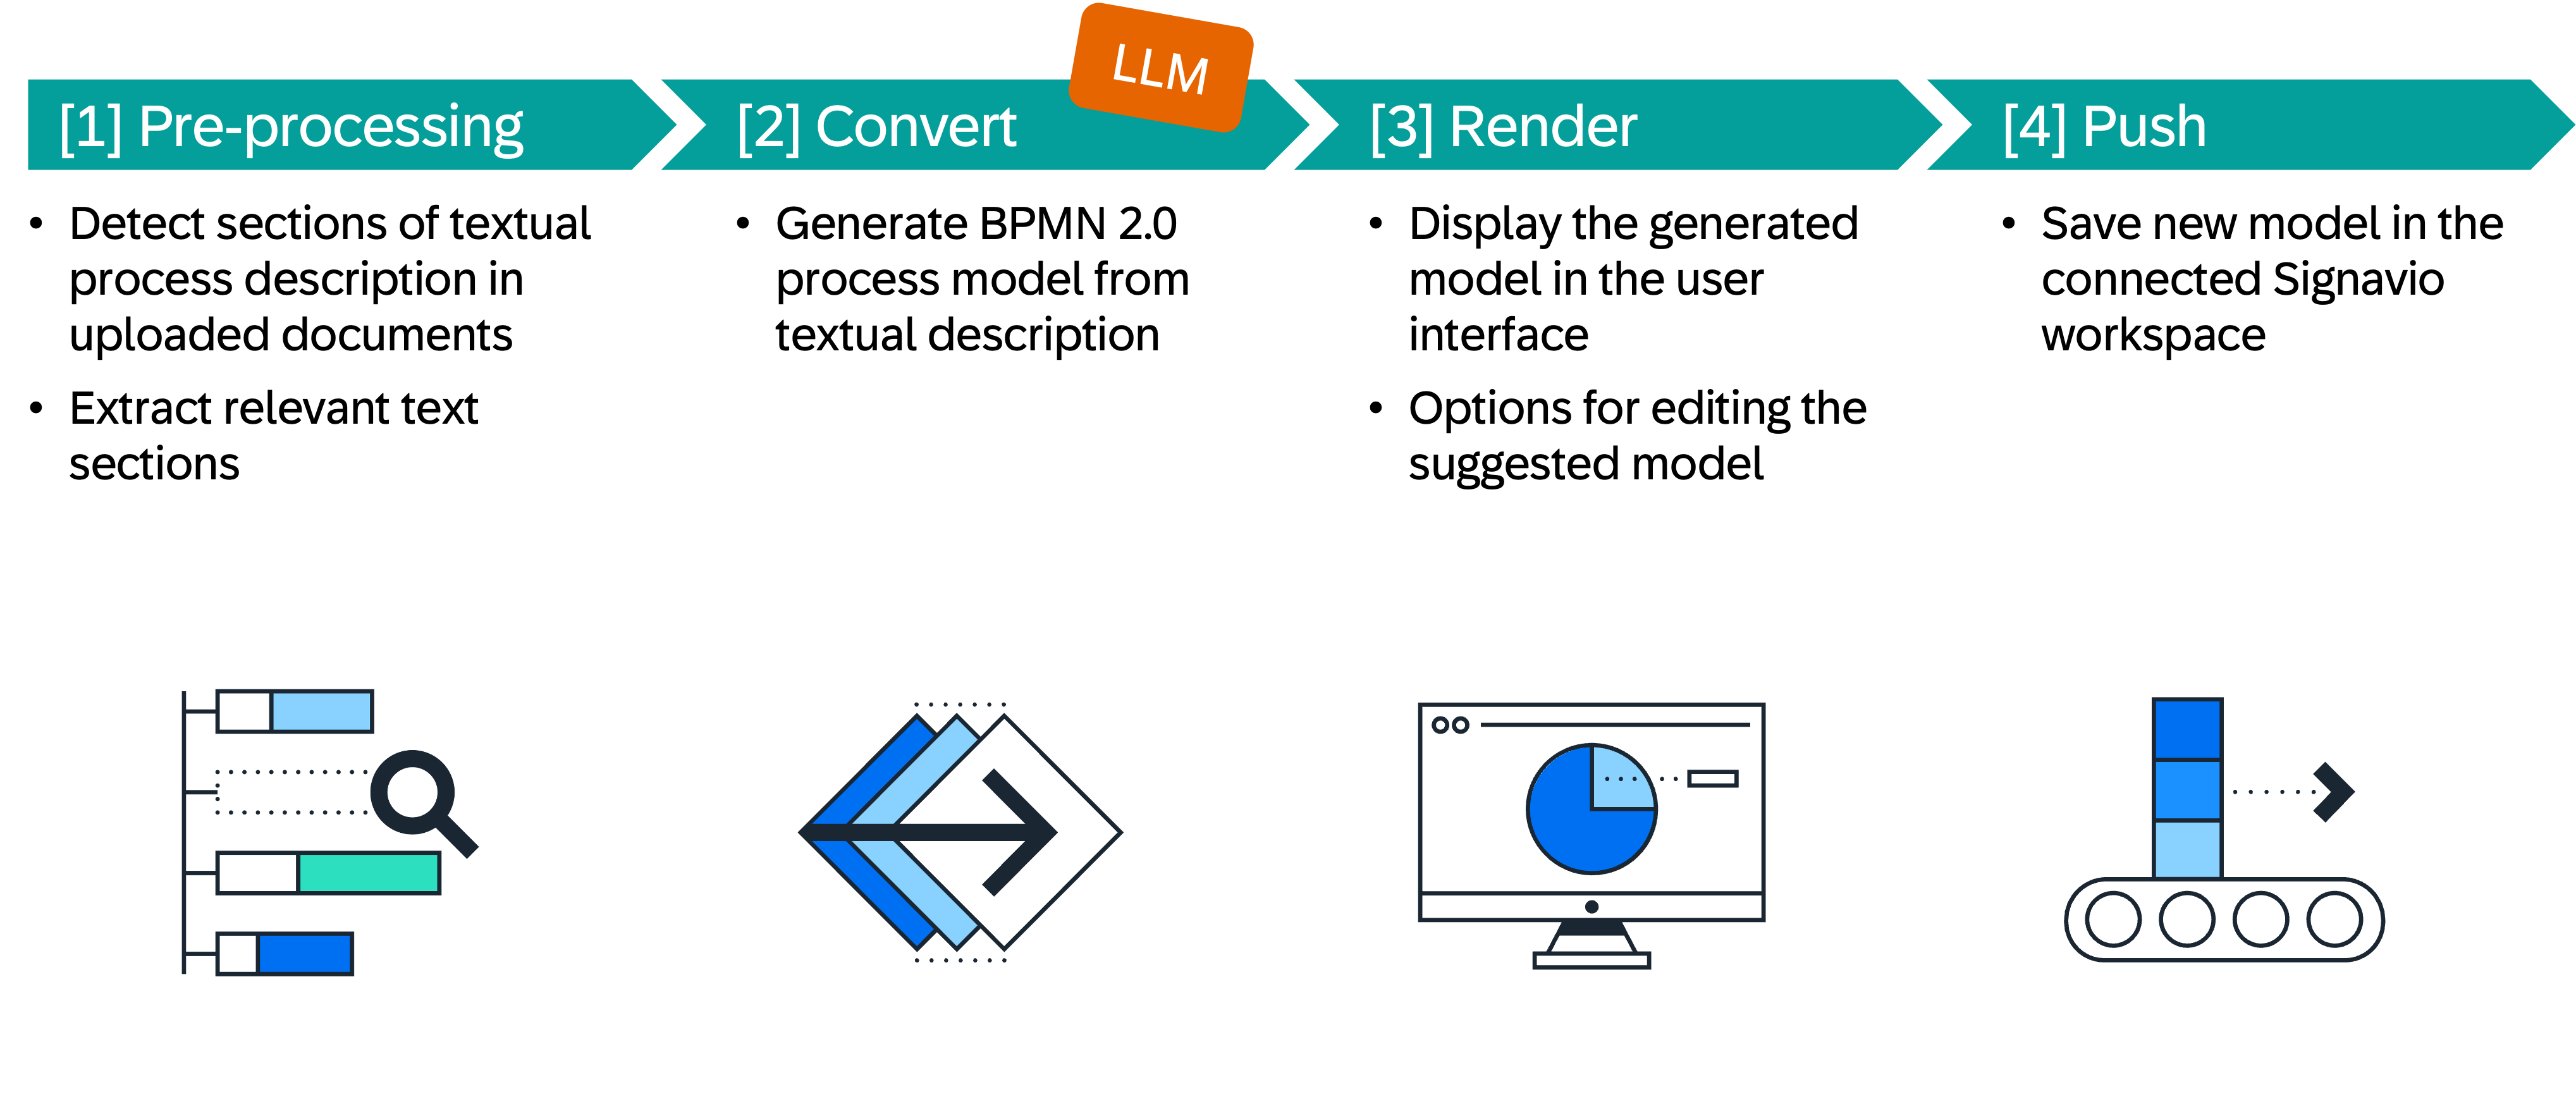
\includegraphics[width=\textwidth,height=\textheight,keepaspectratio]{../assets/images/Text to Model Pipeline.png}
    \caption[Text-to-Model Pipeline Overview]{Text-to-Model Pipeline Overview}
    \label{fig:pipeline-overview}
\end{figure}

\section{Text-to-Model Conversion Step}\label{sec:conversion}
Zooming in on the conversion step of the pipeline - the Text-to-Model transformation - the task can be divided into multiple problems:

\begin{itemize}
    \item Activity extraction
    \item Control flow extraction
    \item Additional information extraction:
          \begin{itemize}
              \item Pools and lanes
              \item Documents
              \item IT-systems
              \item Comments
              \item (Message flow)
          \end{itemize}
    \item \gls{signavio}-compliant output format
    \item Implementation effort (non-functional requirement)
\end{itemize}

\paragraph{Activities \& Control Flow}
First, the essential parts of a \acs{bpmn} 2.0 diagram are activities and the control flow. For the activity extraction, all tasks or subprocesses that are performed in the process need to be identified. Subsequently, an accurate and comprehensive title coherent with the \acs{bpmn} 2.0 guidelines \citep{omg2011bpmn} has to be determined for each activity. For the control flow extraction, the sequence of those activities has to be determined. The control flow can also be split up into multiple branches and joined back together using gateways when different or parallel activity sequences are executed.
% [In that regard, the activity count and control flow complexity should be as minimal as possible to avoid redundant information and duplicate sequence flows.]


\paragraph{Additional Information}\label{par:add-info}
Moreover, the diagram should contain additional information to enhance the information value and detail on certain activities. This feature is not essential for a functioning transformation but would drastically increase the value of the generated diagram. The extraction of the message flow won't be addressed in this work, because it is not of high importance for \gls{signavio} users.

\paragraph{Output Format}
Lastly, to save the process model in the connected \gls{signavio-workspace}, the output must be code for a \acs{bpmn} 2.0 diagram, complying with a certain \gls{signavio}-specific format (see \autoref{fig:code-example} for an example). Therefore, the result of the conversion step cannot be any other format, which might be easier to achieve.

\paragraph{Implementation Effort}
As an additional (non-functional) requirement the implementation effort has to be considered. As the context of this work is an innovation project, the resources for testing and implementing approaches are very limited. The primary objective of the project is the development of a \glsentrylong{poc} and the demonstration of feasibility. Therefore, it is crucial to keep the effort to a minimum.

% \chapter{Related work \& Collaboration}\label{chapter:related-work}
\chapter{Related work}\label{chapter:related-work}
Scientific interest and work on the task of transforming natural language into a formal process representation has existed for over 10 years \citep{process-extraction-from-text}. Various approaches from the \acs{nlp} area were investigated to solve this problem \citep{investigation-text-to-bpmn}. However, with the advancements of \gls{llm} capabilities, the \acs{nlp} area was reformed and new approaches have emerged. Still, not many papers investigating these new approaches were published.

\citeauthor{conversational-process-modelling} explore the topic of chatbot-assisted conversational process modeling \citep{conversational-process-modelling}. Among other aspects, their work includes the extraction of tasks and the control flow from a process description using \glspl{llm} and a proposed set of \acsp{kpi} for comparing generated with ground-truth models in an evaluation step. Other work investigates the extraction of business process elements from text \cite{text-to-bp-elem} and the transformation of textual process information to intermediate formats \cite{text-to-inter-rep}.

% Among discussing my work with other \gls{signavio} researcher, I collaborate with Dr. Timotheus Kampik, Adjunct Associate Professor at the Umeå University in Sweden and Principal Scientist in Residence at \gls{signavio}.


\chapter{Approaches to Text-to-Model}
In this chapter, three approaches using the unique natural language understanding capabilities of \acsp{llm} are presented and assessed.

\section{Direct Translation}\label{sec:direct-translation}
\paragraph{Concept}
The most straightforward approach is to directly transform the given process description into \gls{signavio}-compliant \acs{bpmn} 2.0 \acs{json} code\footnote{This \acs{json} code is how \acs{bpmn} 2.0 diagrams can be represented at \gls{signavio} and used in its software. It therefore is the desired output format.} with a single request to an \gls{llm}. This approach is efficient in terms of implementation effort and runtime.

\paragraph{Results}
To test this approach, \acs{gpt}-4 was one-shot prompted to generate such \gls{signavio}-compliant \acs{json} code given a process description. However, the results were not satisfying as the generated code was not in the specified format. The desired format is very complex as it contains a lot of details about the diagram like specific \acsp{id} and explicit coordinates for each graphical element of the diagram (see \autoref{fig:code-example}). Therefore, the \gls{llm} seems to have trouble with generating compliant code. The approach is not further investigated as it fails to meet a key requirement.

% [There are alternative approaches to the direct translation. For example, specifying a simpler \acs{bpmn} 2.0 \acs{json} output format for the \gls{llm} and transforming the simpler one into the \gls{signavio}-compliant format in a second step. Testing that alternative with the same setup as above and a simliar prompt, \acs{gpt}-4 was able to output the specified simpler format correctly. That second step however would require a lot of effort and therefore was not investigated further as there are limited resources to the project.]

\section{Intermediate Graph Representation}\label{sec:mermaid-approach}
\paragraph{Concept}
Another approach is to transform the process description into another (simpler) intermediate format, such as a graph representation, which is transformed into \gls{signavio}-compliant code in an extra step. This might work better than the first approach because the \gls{llm} only needs to understand the simpler intermediate representation, for example, the format of ``Mermaid.js''\cite{mermaid-js} code (example in Figures \ref{lst:mermaid-example-code} and \ref{fig:mermaid-example-graph}).

\paragraph{Results}
Testing the first step of this approach (see the prompt in \autoref{lst:mermaid-prompt}), \acs{gpt}-4 was able to generate valid code for a Mermaid.js graph, with elements similar to \acs{bpmn} 2.0 (see \autoref{lst:mermaid-test-input} and \autoref{fig:mermaid-test-output} for an example input and output of the first step). As \autoref{fig:mermaid-test-output} demonstrates, there are some flaws in the generated diagram. For example, there are two duplicate sequence flows that could be joined back together using a gateway and there are also missing end nodes. To summarize, the first step requires further optimization, and the second conversion step from the intermediate format to the \gls{signavio}-compliant code is required. It might be a viable approach, but it requires too much effort and therefore won't be further investigated for now.

\section{Generating Traces \& Process Mining}\label{sec:traces}
\paragraph{Concept}
Looking at the generated Mermaid.js graph in \autoref{fig:mermaid-test-output}, the generated diagram isn't a comprehensive process representation but rather displays all possible activity sequences. With this in mind, the idea of the third approach is to generate a unique set of \glspl{trace} from the process description and use a \gls{process discovery algorithm} to extract a process model from that.

In the first step, \acs{gpt}-4 is prompted to extract and output a unique set of \glspl{trace} given the process description. The output is a list of \glspl{trace} (see \autoref{lst:traces-example} for an example), which are then used as an (artificial) \gls{event log} and fed into the ``Split Miner'' \citep{split-miner} algorithm that extracts the process model and returns it as compliant code. The Split Miner algorithm is a state-of-the-art \gls{process discovery algorithm} from 2019 that is implemented in an existing \gls{signavio} service. Therefore, the approach is little effort and always returns \gls{signavio}-compliant \acs{json} code for a \acs{bpmn} 2.0 diagram.

\paragraph{Results}Testing this approach (see the prompt for \gls{trace} extraction in \autoref{lst:traces-prompt}), \acs{gpt}-4 reliably extracts a coherent and unique set of \glspl{trace}; the Split Miner service outputs a \gls{signavio}-compliant diagram (see an exemplary result in \autoref{fig:traces-test-output}).

\begin{figure}[h]
    \centering
    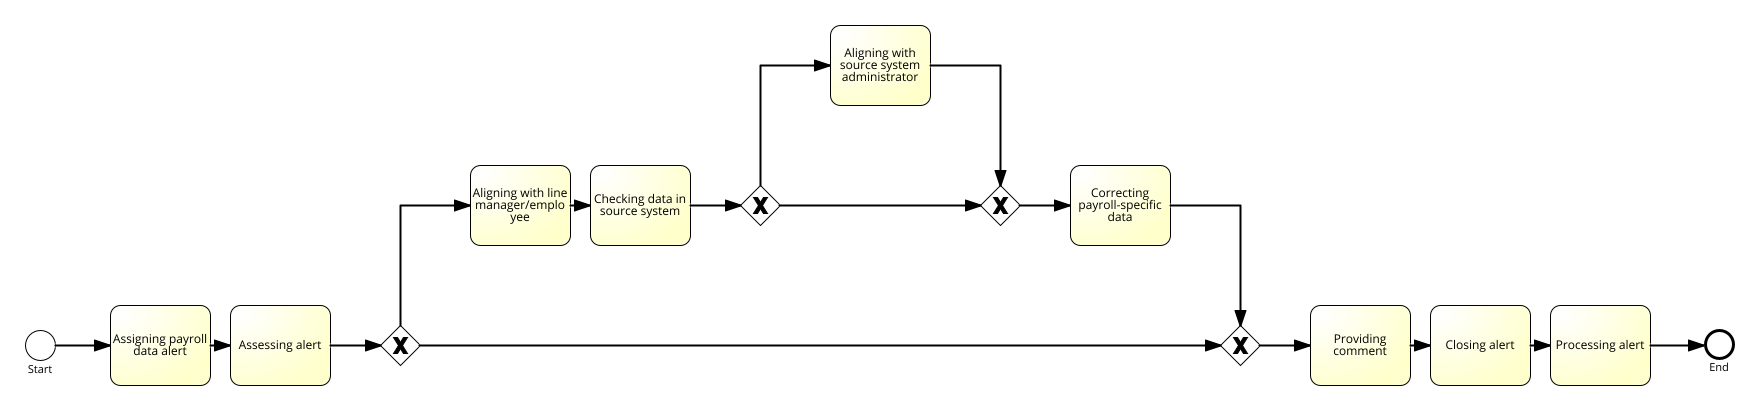
\includegraphics[width=\textwidth,height=\textheight,keepaspectratio]{../assets/images/Traces Test Output.png}
    \caption{Generated \gls{signavio} \acs{bpmn} 2.0 diagram using the \nameref{sec:traces} approach}
    \label{fig:traces-test-output}

    \medskip
    \small
    See the process description used as input in \autoref{lst:traces-test-input} and the generated \glspl{trace} (artificial \gls{event log}) in \autoref{lst:traces-test-traces}.
\end{figure}

For various process descriptions, with similar structure, syntax, and complexity to the one shown in \autoref{lst:traces-test-input}, the output diagram always contains all referenced activities and the correct control flow, represented by activities, exclusive gateways, a start, and an end node.

For process descriptions that are more ambiguous, implicit, and complex (see example in \autoref{lst:hard-description}), the current implementation of the approach struggles to extract complex control flows perfectly. Partially, the assumption of implicit knowledge is missing. However, that doesn't mean it can't deal with more difficult process descriptions, but the approach has to be fine-tuned, e.g. by optimizing prompts and covering certain edge cases.


\chapter{Evaluation}
To systematically assess the performance of any conversion approach, its generated diagram has to be evaluated for various process descriptions of different complexities. The evaluation can be done by an expert in process modeling, who manually compares the generated diagram with the original process description in terms of extracted activities, control flow, and additional information.

If there was a dataset of process descriptions with matching \acs{bpmn} 2.0 diagrams given, another possibility is to compare the diagram generated from the process description with the matching diagram from the dataset. This \textit{round-trip} evaluation can also be performed automatically. Therefore, a set of formal metrics to measure the conformance of the two diagrams need to be defined \cite{bpmn2-comformance, bpmn-event-log-conformance-checking, bpmn-conformance}. This automatic round-trip evaluation could be more accurate by reducing manual errors and biases and would allow different approaches to be formally evaluated as well as each part of an approach to be optimized against an objective score. However, it also requires additional preliminary effort and an appropriate dataset, which is not trivial. For example, many different diagrams are valid ground-truth diagrams for one process description. This especially applies to complex and ambiguous descriptions assuming much implicit knowledge \cite{process-model-ambiguity}.

As the purpose of this work is to investigate approaches that can solve the crucial problems of the described task in the first place, that's how approaches are evaluated. Any further evaluation techniques are not the topic of this work.

\chapter{Prototype Implementation}
The Mermaid.js and \nameref{sec:traces} approaches were implemented as prototypes, showcasing the functionality and the current progress to other internal stakeholders. Both prototypes were built as a web application with Python 3.11 \cite{python3} and the open-source library Streamlit \cite{streamlit}. For using \acs{gpt}-4, both prototypes use \gls{sap}'s \acs{btp} \acs{llm} Proxy Service, \gls{sap}'s service for \acs{llm} usage that uses Microsoft's Azure OpenAI Service \cite{azure-openai} in the background. The Mermaid.js approach prototype can be run locally (see screenshot of the prototype in \autoref{fig:mermaid-prototype}). As the \nameref{sec:traces} approach is more promising, this prototype was made available internally. It is deployed on \gls{sap}'s \gls{btp}, hosted by Cloud Foundry (see screenshot of the prototype in \autoref{fig:trace-prototype}).


\begin{figure}[h]
    \centering
    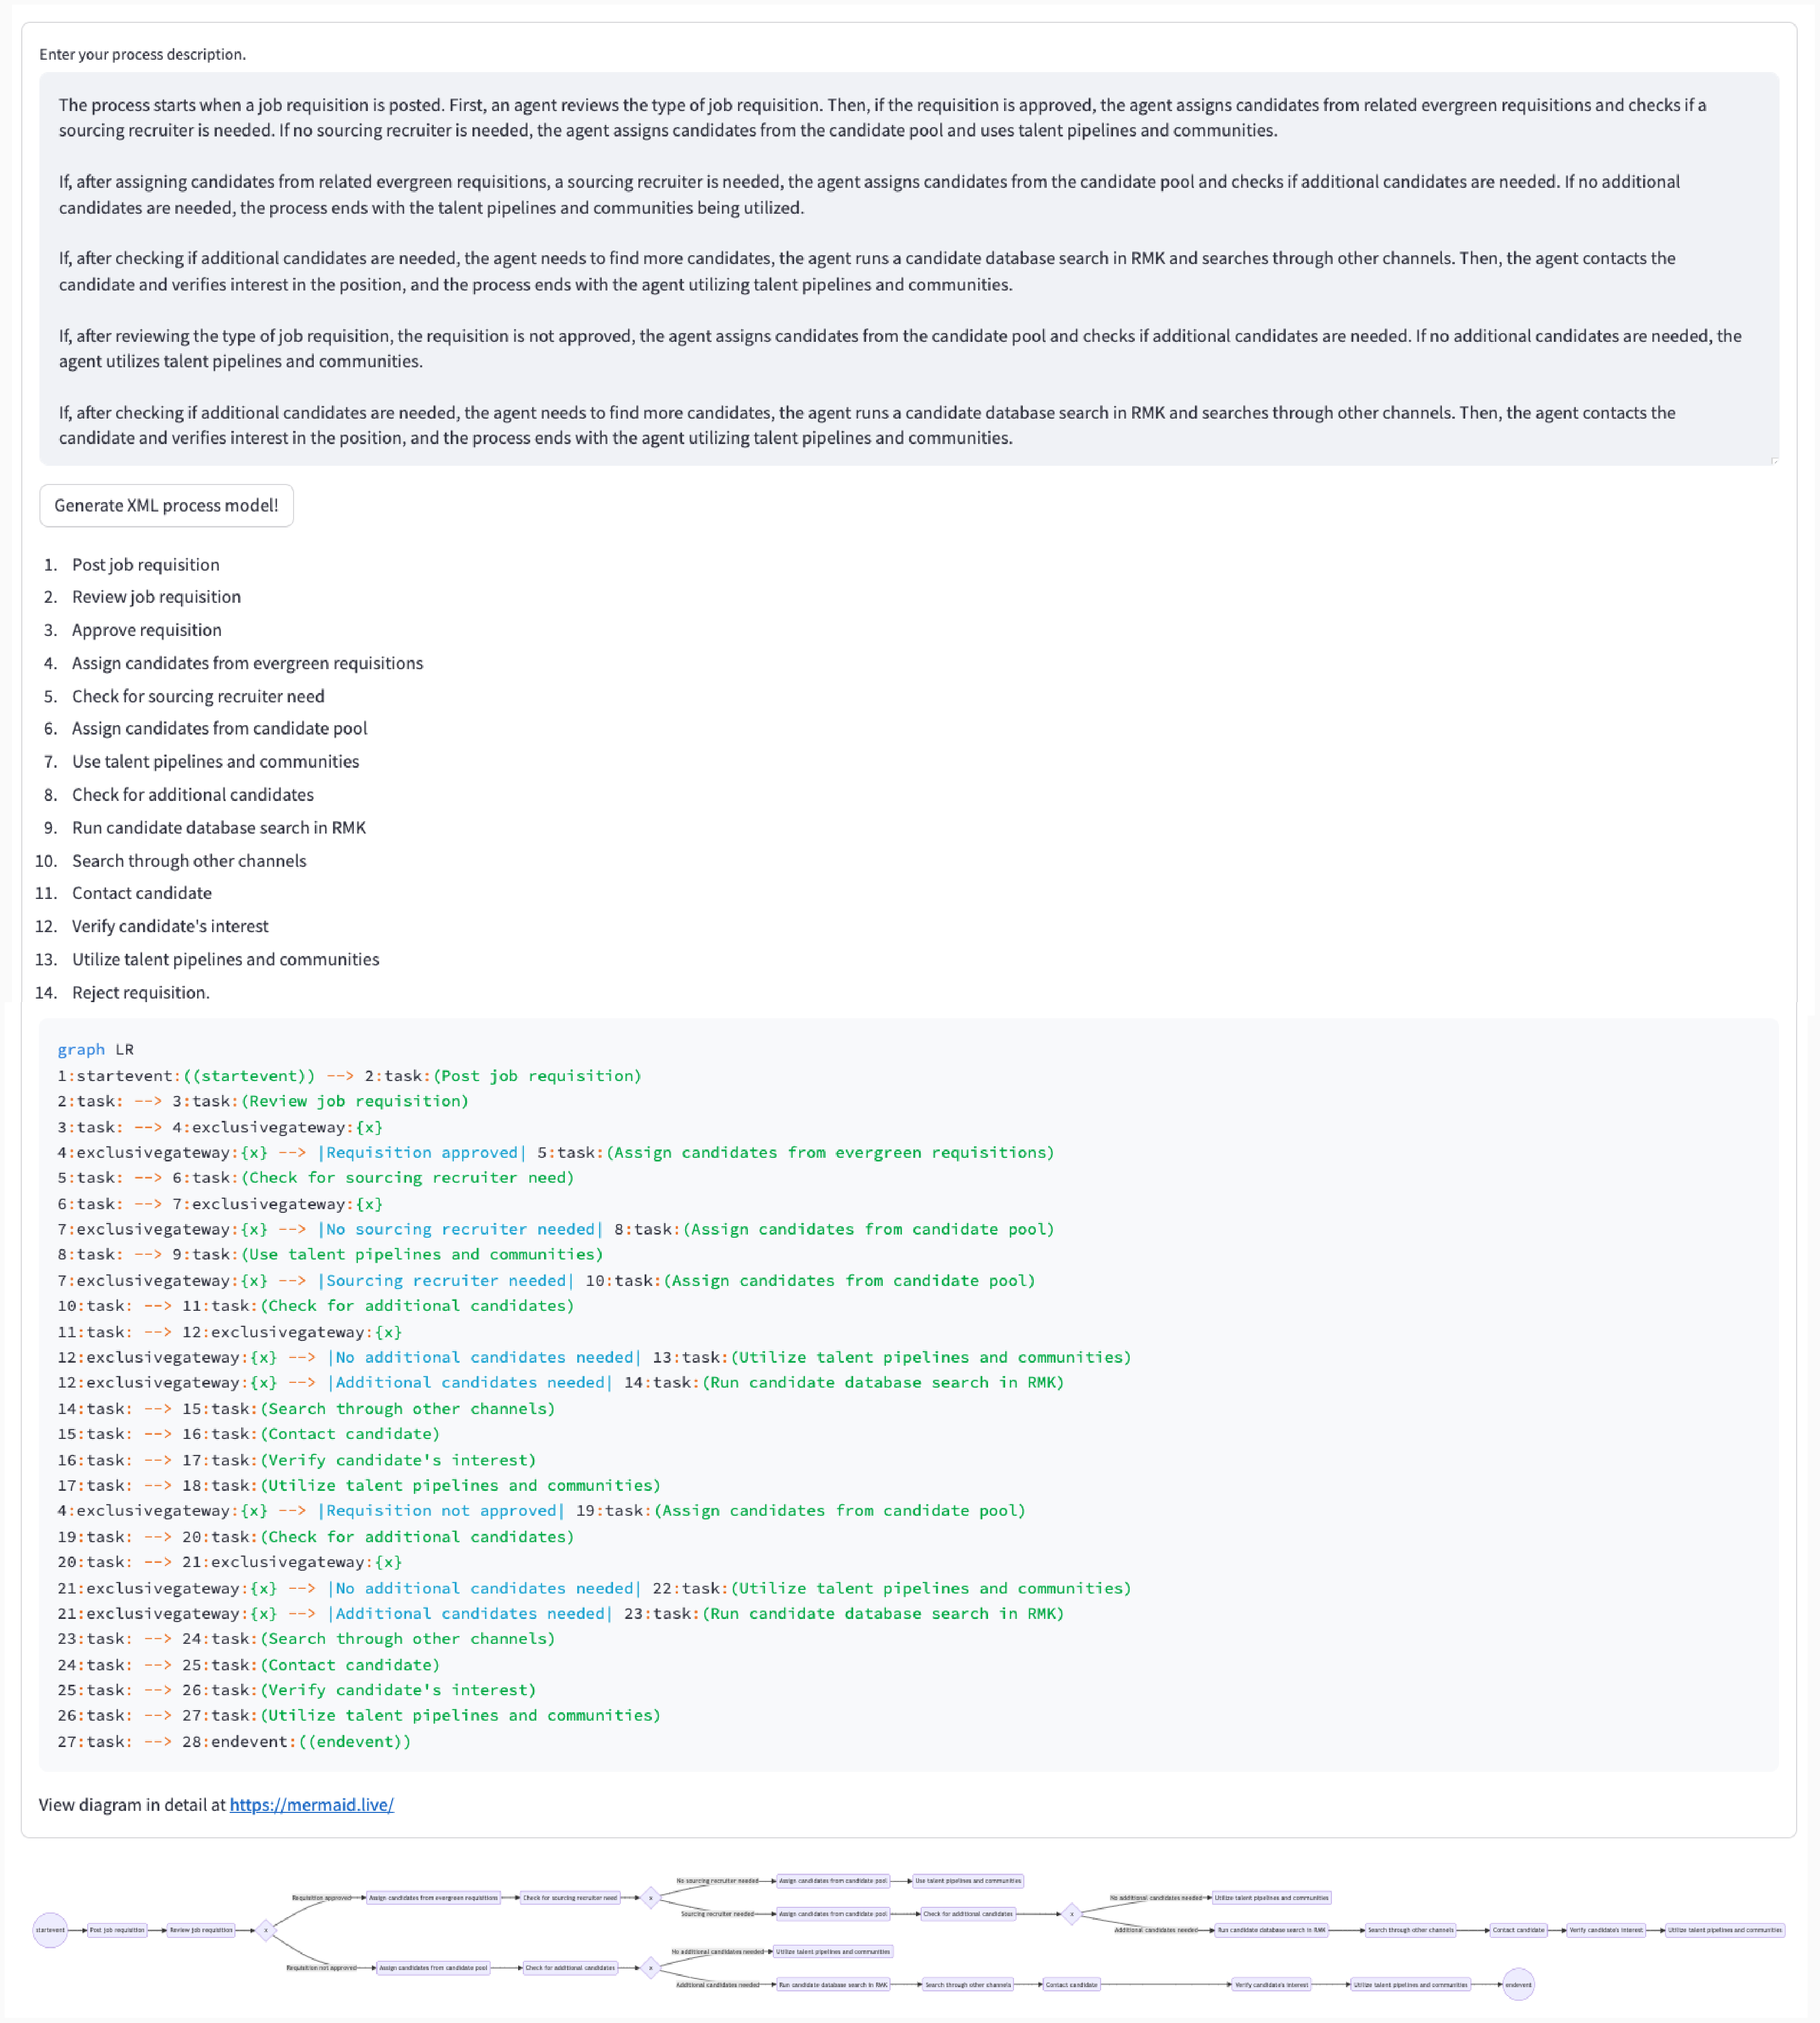
\includegraphics[width=\textwidth,height=\textheight,keepaspectratio]{../assets/images/Mermaid prototype.png}
    \caption{Screenshot of the Mermaid.js approach prototype}
    \label{fig:mermaid-prototype}

    \medskip
    \small
    See the outputted graph also  in \autoref{fig:mermaid-test-output}.
\end{figure}

\begin{figure}[h]
    \centering
    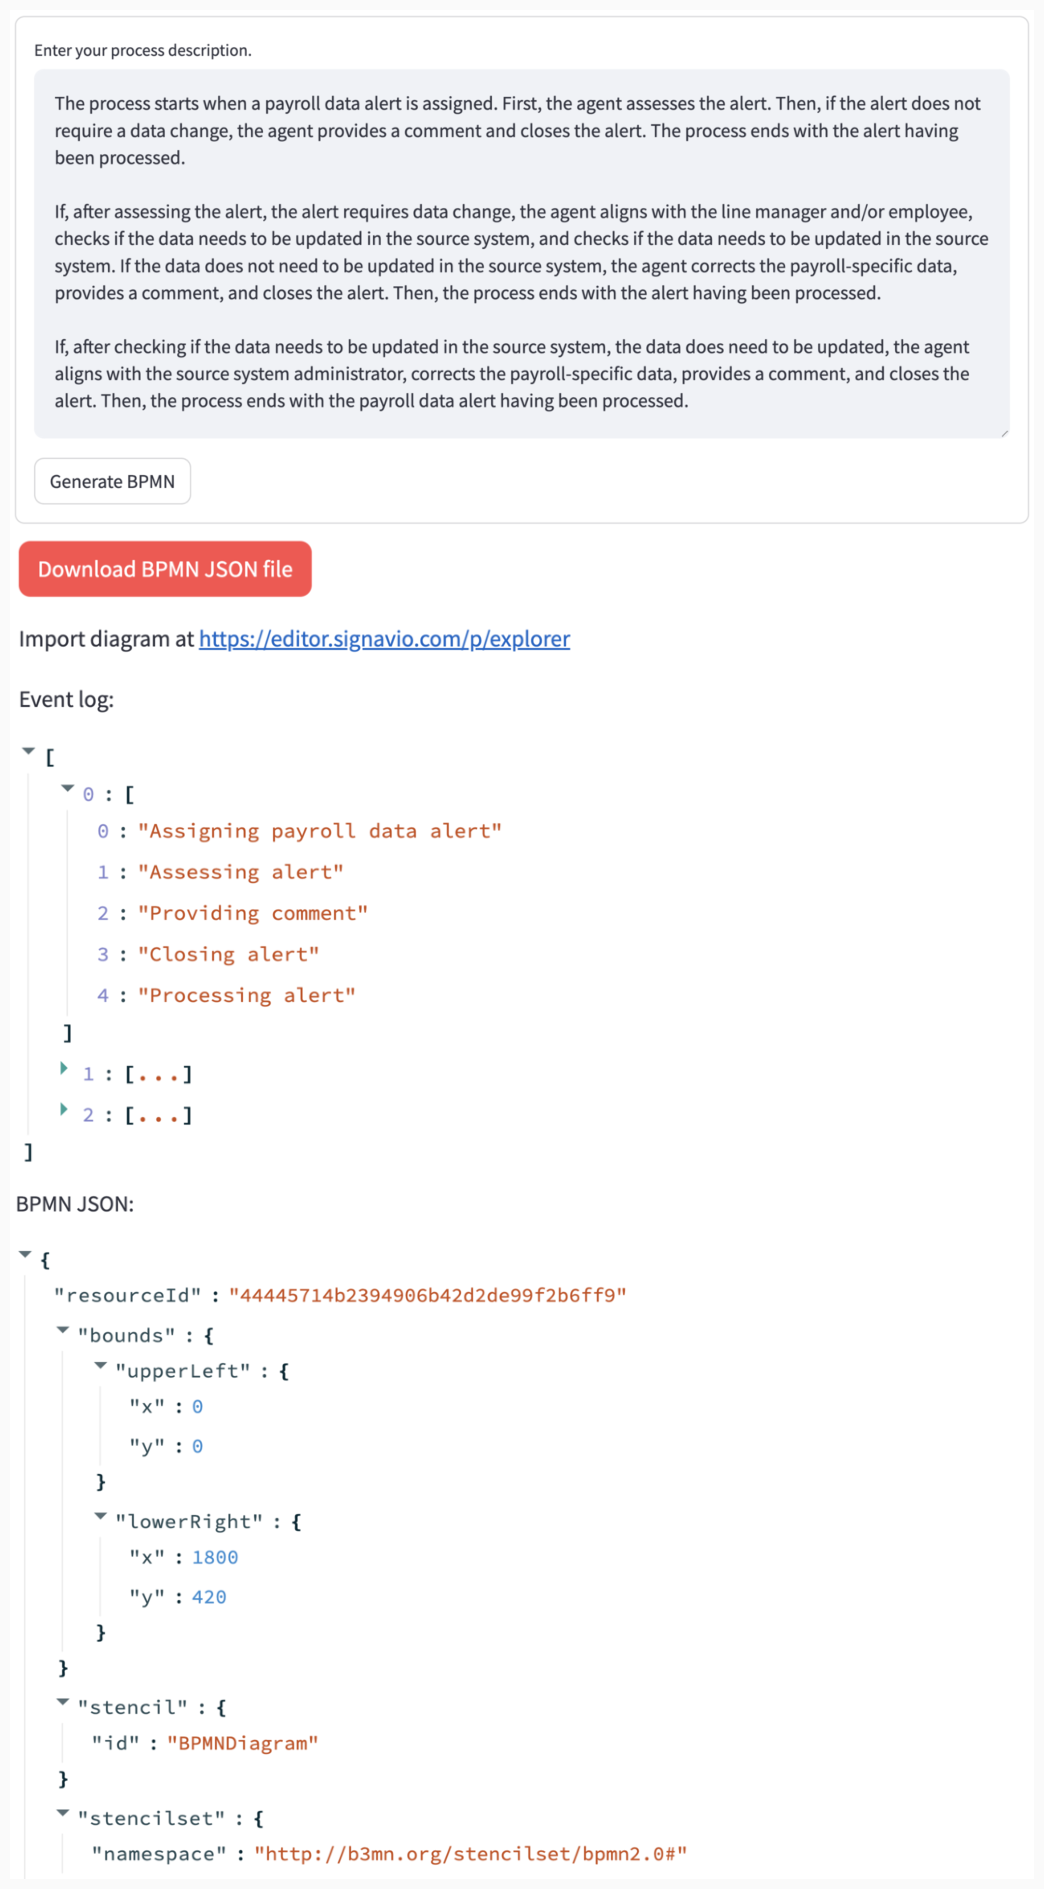
\includegraphics[height=0.95\textheight,keepaspectratio]{../assets/images/Trace prototype.png}
    \caption{Screenshot of the \nameref{sec:traces} approach prototype}
    \label{fig:trace-prototype}

    \medskip
    \small
    See the outputted diagram in \autoref{fig:traces-test-output}.
\end{figure}

\chapter{Discussion}
\paragraph{Summary}
Aggregating all results, the approaches \nameref{sec:direct-translation} and \nameref{sec:mermaid-approach} are not suitable for the current \acs{poc} project. However, the \nameref{sec:traces} approach solves all the crucial problems of the task. It extracts the activities and the control flow and always outputs \gls{signavio}-compliant \acs{bpmn} 2.0 \acs{json} code. The approach is also very efficient in terms of implementation effort as all its functionality is handled by two existing services (\acs{gpt}-4 and the \gls{signavio} Split Miner service). Meanwhile, it does not extract additional information as described in the \hyperref[par:add-info]{problem statement} and still struggles with more difficult process descriptions. But, the approach also leaves room for further development and improvement (see \nameref{par:next-steps}). It therefore is a viable solution for the development of a \acs{poc}.


\paragraph{Future Work}\label{par:next-steps}
Some next steps regarding the \nameref{sec:traces} approach that can be the subject of future work are:

\begin{itemize}
    \item Add a post-processing step to enhance the diagram with additional information using another \gls{llm} request, given the process description and generated diagram code
    \item Gather more (diverse) process descriptions to systematically examine edge cases and malfunctions
    \item Implement an automated round-trip evaluation after defining a set of formal metrics
    \item Optimize the used prompts and assess the application of prompt chaining
    \item Experiment with human-in-the-loop approaches:
          \begin{itemize}
              \item Suggest multiple possible process variants and allow the user to select
              \item Allow the user to edit extracted \glspl{trace}, following conversational modeling \cite{conversational-process-modelling}
          \end{itemize}
\end{itemize}

The work, presented in this report will be continued and advanced.

% add: survey about most used BPMN components / elements, add to section above that explains that message flow is not that important